\documentclass{article}
\usepackage[utf8]{inputenc}
\usepackage[french]{babel}
\usepackage[T1]{fontenc}
\usepackage[hidelinks]{hyperref}

\usepackage{amsmath}
\usepackage{amssymb}
\usepackage{graphicx}
\usepackage{listings}
\usepackage{color}

\begin{document}

\begin{titlepage}
    \begin{center}
        
        {\Large Université de Mons}\\[1ex]
        {\Large Faculté Des Sciences}\\[1ex]
        
        \newcommand{\HRule}{\rule{\linewidth}{0.3mm}}
        % Title
        \HRule \\[0.5cm]
        { \LARGE \bfseries Réseaux 1 \\[0.3cm]}
        { \LARGE \bfseries Rapport : Selective Repeat \& Congestion \\[0.1cm]} % Commenter si pas besoin
        { \LARGE \bfseries Groupe 9 \\ [0.05cm]}
        \HRule \\[1.5cm]
        
        % Author and supervisor
        \begin{minipage}[t]{0.45\textwidth}
            \begin{flushleft} \large
                \emph{Professeur:}\\
                Bruno \textsc{Quoitin}\\
                \emph{Assistants:}\\
                Jeremy \textsc{Dubrulle}\\
            \end{flushleft}
        \end{minipage}
        \begin{minipage}[t]{0.45\textwidth}
            \begin{flushright} \large
                \emph{Auteurs:} \\
                Cyril \textsc{Moreau} (210376)\\
                Arnaud \textsc{Moreau} (211260)\\
            \end{flushright}
        \end{minipage}\\[2ex]
        
        \vfill
        
        % Bottom of the page
        \begin{center}
            \begin{tabular}[t]{c c c}
                
\includegraphics[height=1.5cm]{UMONS-Logo.jpg} &
                
\includegraphics[height=1.5cm]{FS-Logo.jpg} &
                %\hspace{0.3cm} &
            \end{tabular}
        \end{center}~\\
        
        {\large Année académique 2021-2022}
        
    \end{center}
\end{titlepage}

\newpage

\section{Construction et exécution}
\subsection{Simulateur}
Pour compiler le programme, veuillez exécuter la commande suivante dans le dossier racine :
\begin{verbatim}
    javac -d build reso/examples/selectiveRepeat/Demo.java
\end{verbatim}
Ensuite, pour exécuter le logiciel, veuillez exécuter la commande depuis le dossier \textit{build} créé :
\begin{verbatim}
    java reso/examples/selectiveRepeat/Demo
\end{verbatim}
Une fois l'application lancée, il faudra entrer le nombre de paquet à envoyer, la probabilité de perte
de paquet ou de acknowledgement, mais aussi le \textit{bit rate} du lien et la longeur du lien (en km).
\begin{figure}[h]
    \centering 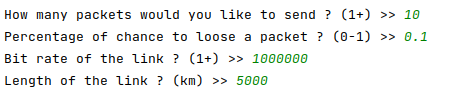
\includegraphics[scale=0.5]{data.png}
    \caption{Exemple de paramètres}
\end{figure}

\subsection{Création de plot pour la taille de la fenêtre}
Après avoir exécuté l'application, un fichier \emph{WindowSize.csv} est créé contenant
un historique des modifications de la taille de la fenêtre d'envoi.
Deux script python sont fournis afin de permettre de visualiser ces changement.
Le premier utilisant \emph{plotly} et le deuxième \emph{matplotlib}.
Afin de faire fonctionner ces script, veuillez installer les librairies suivantes : 
\begin{center}
    \begin{verbatim}
        pip install pandas
        pip install plotly (premier script)
        pip install matplotlib (deuxième script)
    \end{verbatim}
\end{center}
\textbf{Attention} le fichier \textit{WindowSize.csv} doit être dans le même dossier que le script.
Pour éxécuter un des script, il suffit d'exécuter l'une de ces commandes :
\begin{center}
    \begin{verbatim}
        python plot.py
        python plot2.py
    \end{verbatim} 
\end{center}

\end{document}